% TODO before submission:
%  - Fill in the author name/affiliation in \author{} (marked with <<< >>>)
%  - Verify the meeting/venue line if the conference mandates one
\documentclass[conference]{IEEEtran}
\IEEEoverridecommandlockouts

\usepackage{cite}
\usepackage{amsmath,amssymb,amsfonts}
\usepackage{graphicx}
\usepackage{textcomp}
\usepackage{xcolor}
\usepackage{tikz}
\usetikzlibrary{arrows.meta,positioning,fit,calc,backgrounds}
\usepackage{url}
\def\BibTeX{{\rm B\kern-.05em{\sc i\kern-.025em b}\kern-.08em T\kern-.1667em\lower .7ex\hbox{E}\kern-.125emX}}

\graphicspath{{figures/}{../imgs/}}

\begin{document}

\title{A Low-Cost Semi-Autonomous Rover for Laser Weed Control\\
with Smartphone-Based Field Mapping}

% <<< TODO: replace with the real author name and affiliation >>>
\author{
\IEEEauthorblockN{Bayazid Habib Siddikee}
\IEEEauthorblockA{Dept.~of Mechatronics Engineering\\
Rajshahi University of Engineering \& Technology (RUET)\\
Rajshahi, Bangladesh\\$<$email$>$}
}

\maketitle

\begin{abstract}
 Herbicide-resistant weeds, residue regulations, and the rising cost of manual
 weeding create pressure for non-chemical weed control on smallholder farms,
 where commercial laser-weeding platforms are prohibitively expensive. This
 paper presents a low-cost semi-autonomous weeding rover that plans missions
 from a single smartphone photograph: the operator taps the four corners of a
 field block in the app, and the rover's embedded computer warps the photo into
 a metric top-down (bird's-eye-view) image, segments vegetation using an
 excess-green threshold with Otsu-backed automation, extracts crop rows by
 column projection, regularizes them against the operator-declared row count,
 and emits a boustrophedon waypoint mission that a 3-DOF targeting arm follows
 to aim the laser. The perception step is quantitatively evaluated on a
 reproducible synthetic benchmark spanning camera tilt, row pitch, and
 corner-tapping error. Regularized row extraction restored exact row-count
 detection in \textbf{100\,\%} of trials at tilts up to $60^\circ$, whereas the
 unregularized pipeline dropped to 75\,\% at $50$--$60^\circ$ on a tight
 0.6\,m row pitch. Row position error remained below 8\,cm at $60^\circ$, and
 the complete real-photo pipeline ran in 19.5\,ms per field block. All
 software stages are validated end-to-end in a physics-visualized 3-D tandem
 simulation, and the system is embodied in a working chassis prototype with a
 full KiCad electrical design.
\end{abstract}

\begin{IEEEkeywords}
 weeding robot, laser weeding, precision agriculture, bird's-eye view,
 row detection, low-cost robotics, embedded vision
\end{IEEEkeywords}

\section{Introduction}
Weeds are a primary cause of crop-yield loss, and their control still relies
heavily on manual labor or herbicide programs whose residue and resistance
drawbacks are increasingly difficult to sustain~\cite{oerke2006}. Laser
weeding is an attractive non-chemical alternative: a focused beam damages weed
meristems within a fraction of a second, leaves no residue, and requires no
contact with the crop. However, reported systems---academic platforms built on
high-end field robots~\cite{ruckelshausen2009,wu2020} and commercial units
such as the Carbon LaserWeeder~\cite{carbonrobotics}---target large farms and
remain far outside the budget envelope of smallholder agriculture.

Between these poles sits a gap: semi-autonomous rovers that borrow human
judgment where it is cheap (one photograph per field block, taken with a
commodity smartphone) and automate what is expensive or dangerous
(navigation, repeatability, laser aiming). Prior vision-based weeding robots
demonstrated row tracking from an on-board camera~\cite{astrand2002}, but
typically assume continuous in-motion perception. Our requirements differ:
targeted laser work needs an accurate global lane map \emph{before} the rover
enters the field, and the only sensor guaranteed to be available to a
smallholder is a phone camera.

This paper makes the following contributions:
\begin{enumerate}
  \item A complete, low-cost architecture for laser weeding in which a
        smartphone photo plus four corner taps is the sole mission-autonomy
        input, processed on a Raspberry Pi-class single-board computer
        (Section~\ref{sec:system}).
  \item A field-perception pipeline that is deliberately robust to arbitrary
        handheld camera pose, built around a corner-driven bird's-eye-view
        (BEV) warp and an expected-count row regularizer, with a quantitative
        account of why tilts degrade raw projection and how
        regularization removes that failure mode
        (Sections~\ref{sec:perception} and~\ref{sec:eval}).
  \item A reproducible synthetic-field robustness benchmark (camera tilt,
        row pitch, corner-tap noise) and a real-photo timing characterization,
        released as runnable artifacts with the system
        (Section~\ref{sec:eval}).
  \item An end-to-end 3-D tandem simulation whose replay drives the same
        waypoints and zap decisions the hardware executes, plus a physical
        chassis prototype and a connectivity-verified KiCad electrical
        design (Sections~\ref{sec:electrical} and~\ref{sec:mission}).
\end{enumerate}

\section{System Architecture}\label{sec:system}

\begin{figure}[t]
\centering
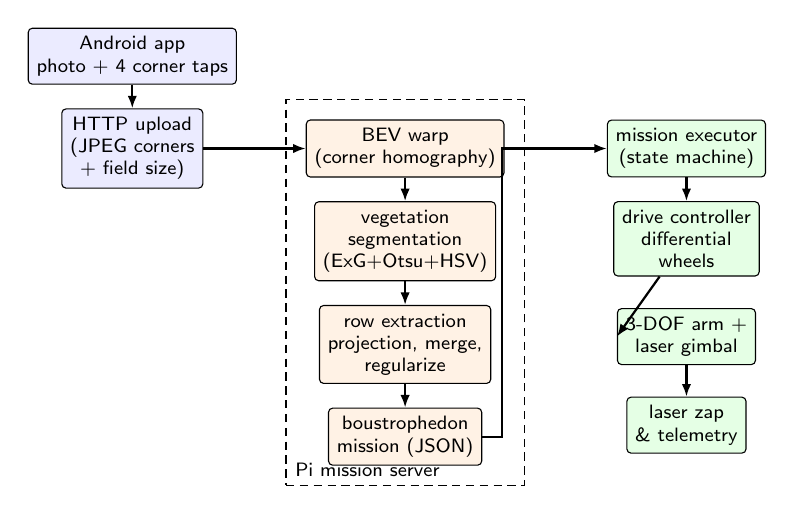
\begin{tikzpicture}[
  font=\scriptsize\sffamily, node distance=3mm,
  box/.style={draw, rounded corners=1.5pt, align=center, inner sep=3pt,
              minimum height=5.5mm, fill=white},
  src/.style={box, fill=blue!8},
  pi/.style={box, fill=orange!10},
  hw/.style={box, fill=green!10},
  arr/.style={-{Latex[length=1.6mm]}, thick}]
% left column: phone
\node[src] (phone) {Android app\\photo + 4 corner taps};
\node[src, below=of phone] (http) {HTTP upload\\(JPEG corners\\+ field size)};
% middle: pi pipeline
\node[pi, right=13mm of http] (warp) {BEV warp\\(corner homography)};
\node[pi, below=of warp] (seg) {vegetation\\segmentation\\(ExG+Otsu+HSV)};
\node[pi, below=of seg] (rows) {row extraction\\projection, merge,\\regularize};
\node[pi, below=of rows] (plan) {boustrophedon\\mission (JSON)};
% right: hardware
\node[hw, right=13mm of warp] (exec) {mission executor\\(state machine)};
\node[hw, below=of exec] (drive) {drive controller\\ differential\\wheels};
\node[hw, below=of drive, yshift=-1mm] (arm) {3-DOF arm +\\laser gimbal};
\node[hw, below=of arm, yshift=-1mm] (zap) {laser zap\\\& telemetry};
% arrows
\draw[arr] (phone) -- (http);
\draw[arr] (http) -- (warp);
\draw[arr] (warp) -- (seg);
\draw[arr] (seg) -- (rows);
\draw[arr] (rows) -- (plan);
\draw[arr] (plan.east) -- ++(2.5mm,0) |- (exec.west);
\draw[arr] (exec) -- (drive);
\draw[arr] (drive) -- (arm.west);
\draw[arr] (arm) -- (zap);
% enclosing Pi box
\begin{scope}[on background layer]
  \node[draw, densely dashed, fit=(warp)(seg)(rows)(plan),
        inner sep=2.5mm, label={[anchor=south west]south west:Pi mission server}] {};
\end{scope}
\end{tikzpicture}
\caption{System architecture. The phone contributes exactly one photograph
and four corner taps; all perception, planning, and execution happens
on the rover's on-board computer.}
\label{fig:arch}
\end{figure}

\subsection{Hardware Platform}
The rover chassis is a four-wheel differentially driven platform carrying an
RPi-class single-board computer that hosts the mission server, an ESP32
acting as the real-time motor bridge, and an ultrasonic proximity sensor for
headland safety stop. Above the chassis sits a 3-DOF arm: two continuous-axis
servos orient a laser diode in pan and tilt, and the third servo deploys/masks
the beam through a gimbal-mounted pointer. The complete electrical system is
described in Section~\ref{sec:electrical}; it was machine-generated as a
fully-wired KiCad sheet and gated on netlist/ERC verification.

\subsection{Electrical Design}\label{sec:electrical}
The complete electrical system was drawn in KiCad 9 as a generated,
fully-wired single sheet: a 3S LiPo feeds a main switch and 15\,A fuse into a
shunt-monitored 12\,V rail (INA219 over I$^2$C), a 5\,V buck powers the
Pi-class SBC, a dedicated 6\,V UBEC rail powers the arm servos in isolation,
dual MD13S bridges drive the wheel groups, and the laser line runs through a
hardware key-lock interlock that the on-board computer's laser-enable signal
must logically AND with before the driver stage fires. Two HC-SR04
ultrasonics and two VL53L0X ToF sensors provide front and rear proximity
sensing, and an emergency-stop button breaks the laser enable and motor
command chain. Every pin of every component bears its net label, so net
connectivity is anchored by labels even where a route is drawn only
logically; the exported netlist reproduces all 37 named nets exactly as
designed---this was not the case for an earlier revision, whose routing pass
allowed different nets to share wire cells and thereby merged most of the
sheet into a single net, a failure mode caught exactly by this verification
gate and fixed by claiming cells exclusively during routing. ERC on the fixed
sheet reports zero connectivity violations (the remaining notices concern the
symbol-library table, a configuration matter). Fig.~\ref{fig:schematic} shows
the result; the KiCad source, PDF export, and netlist ship with the
repository artifacts.

\begin{figure}[t]
\centering
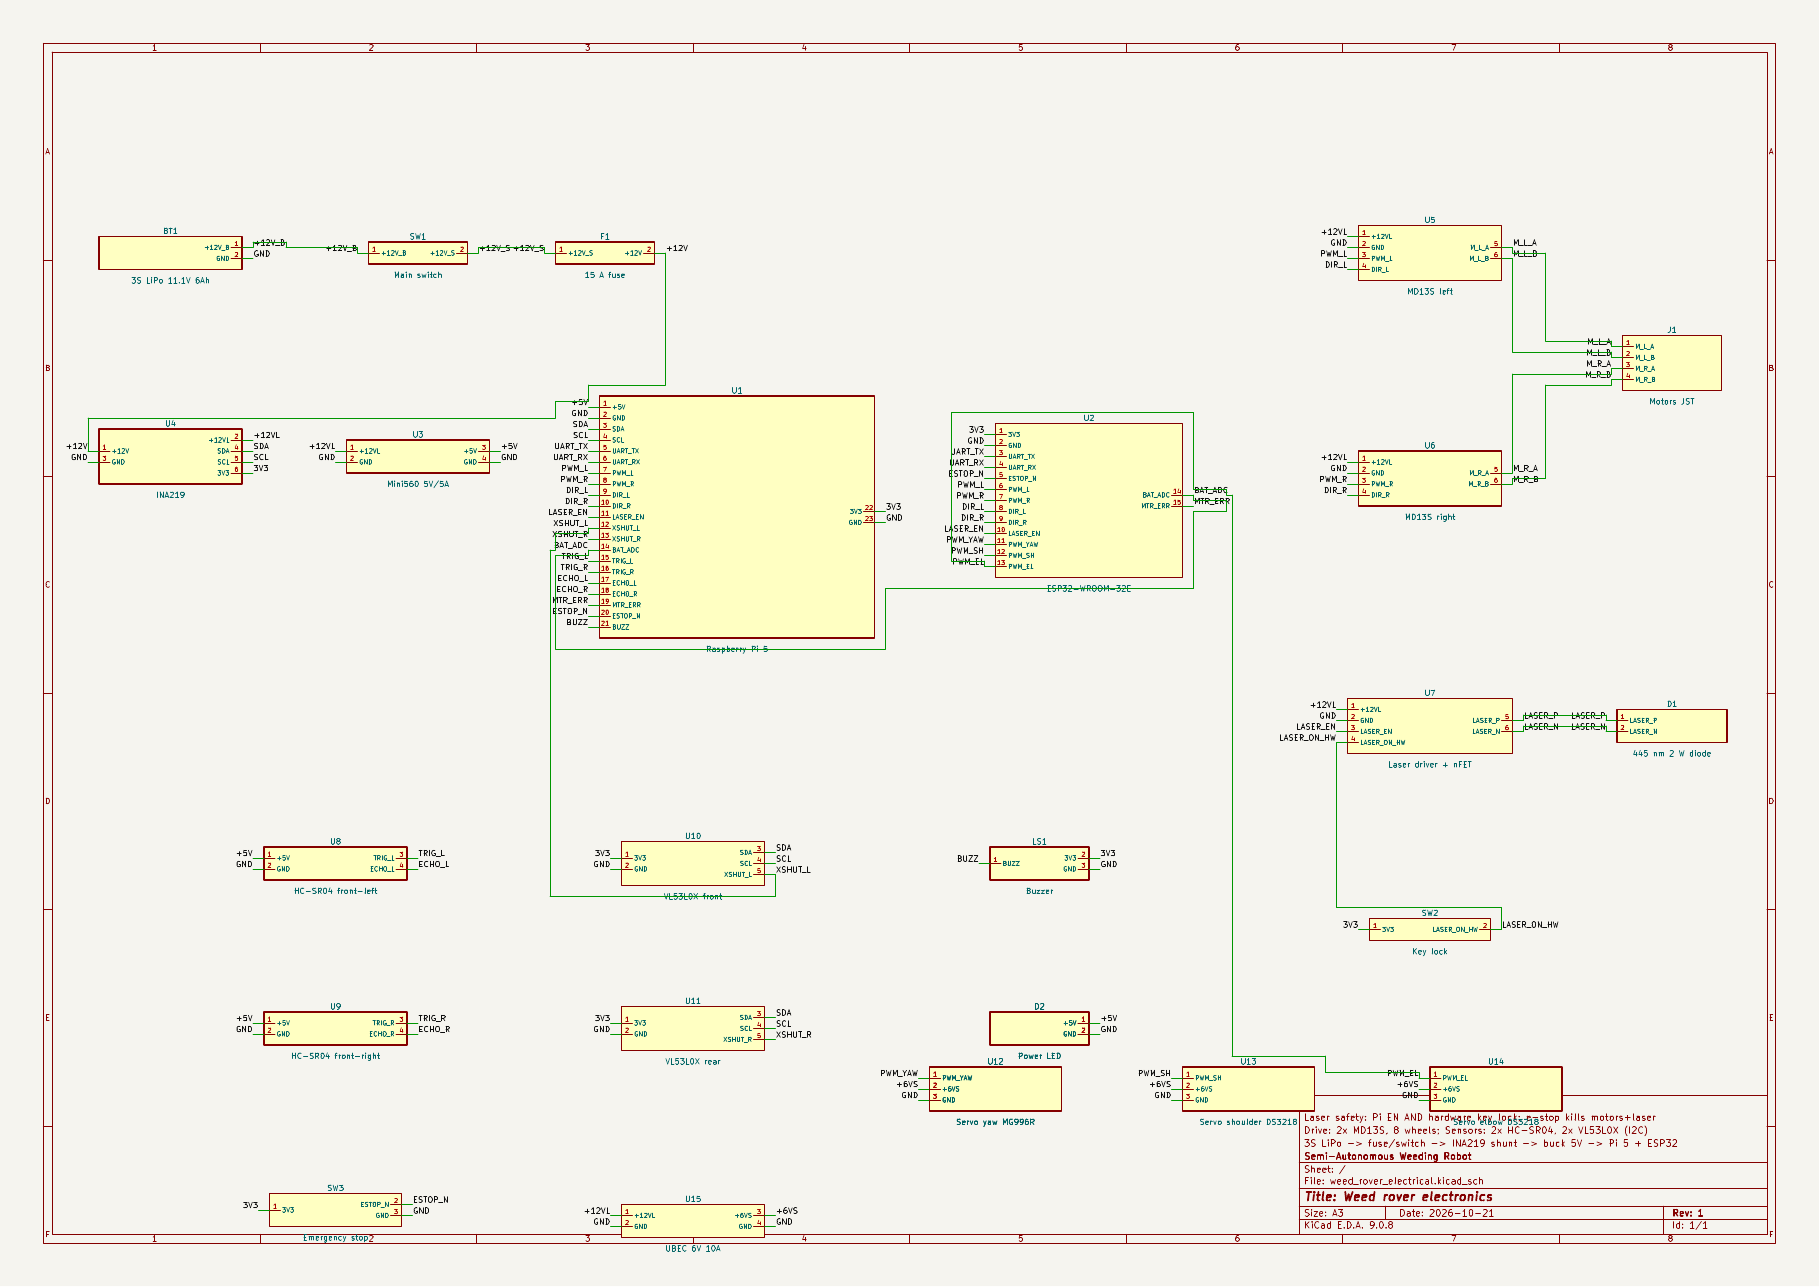
\includegraphics[width=\linewidth, angle=90]{weed_rover_schematic.png}
\caption{Complete KiCad electrical schematic of the rover. Net labels at
every pin keep connectivity legible; netlist export and ERC serve as the
verification gate.}
\label{fig:schematic}
\end{figure}

\subsection{Software Organization}
The pipeline is deliberately split at exactly one boundary: a JSON/HTTP
exchange between the phone app and the rover. The app uploads a JPEG image,
the four tapped corners in photo coordinates, and the field's physical
dimensions (width, length, and the operator's row count). Everything
downstream---warping, segmentation, row extraction, mission planning,
execution, and laser control---lives on the rover, so perception parameters
can be retuned per crop without shipping a new phone application.

\section{Field Perception Pipeline}\label{sec:perception}

\subsection{Corner-Driven BEV Warp}
Rather than requiring a nadir (top-down) photograph, the pipeline accepts any
handheld framing: the four tapped corner points, ordered top-left, top-right,
bottom-right, bottom-left, define a field quadrilateral in the photo, which
is warped with a single projective transform into a BEV image of
$900$\,px width scaled to the field's real aspect ratio. Corner-driven
homography recovers the plane geometry exactly, so the \emph{geometric}
tolerance of the method reproduces the skill of a human operator; robustness
to camera tilt is bounded not by geometry but by the \emph{image-quality}
consequences of tilt---the remaining sections show that the perception
stages, not the warp, bear that burden.

\subsection{Vegetation Segmentation}
Vegetation is segmented using the classical excess-green quantity
$E_xG = 2g - r - b$~\cite{woebbecke1995}, whose threshold is chosen
automatically by Otsu's method~\cite{otsu1979} on a contrast-scaled version of
the index, then intersected with an HSV green-dominance test and subjected to
morphological opening/closing to stabilize against soil noise. On the real
field photograph used in Section~\ref{sec:eval}, this stage is both the most
expensive and the most decision-dense step: it fixes the vegetation ratio
that anchors all downstream row reasoning.

\subsection{Row Extraction with Expected-Count Regularization}\label{sec:rows}
Rows are extracted from the BEV's column-wise projection of the vegetation
mask. Segments above 25\,\% of the projection maximum are candidate rows;
short segments are merged when their gap is below $0.6\times$ the expected
row pitch, and their centers are the raw row estimates. Raw projection is
fragile for two reasons: photographs taken at an oblique angle compress the
far edge of the field, spreading blur and JPEG artifacts over several
centimeters of ground sampling distance, and thin row bands can dip below the
projection threshold in gaps between plants and reappear after merging. The
regularizer exploits the one piece of agronomic knowledge nobody on-site
lacks: the crop was planted with an approximately constant row pitch, and
usually a row count the operator knows. Given the expected count $k$, the
regularizer snaps the row centers to a uniform $k$-slot grid that best
matches the detected set---anchored in the median row spacing---so a row
merged into a neighbor or lost to a gap is restored symmetrically around the
failed band rather than left out.

\subsection{Worked Example on a Real Photograph}
Fig.~\ref{fig:realfield} shows the pipeline on an authentic field photo: (a)
the operator-visible scene, (b) the BEV computed from the block corners, and
(c) the final row overlay: 7 of 7 rows detected, as discussed quantitatively
in Section~\ref{sec:eval}.

\begin{figure}[t]
\centering
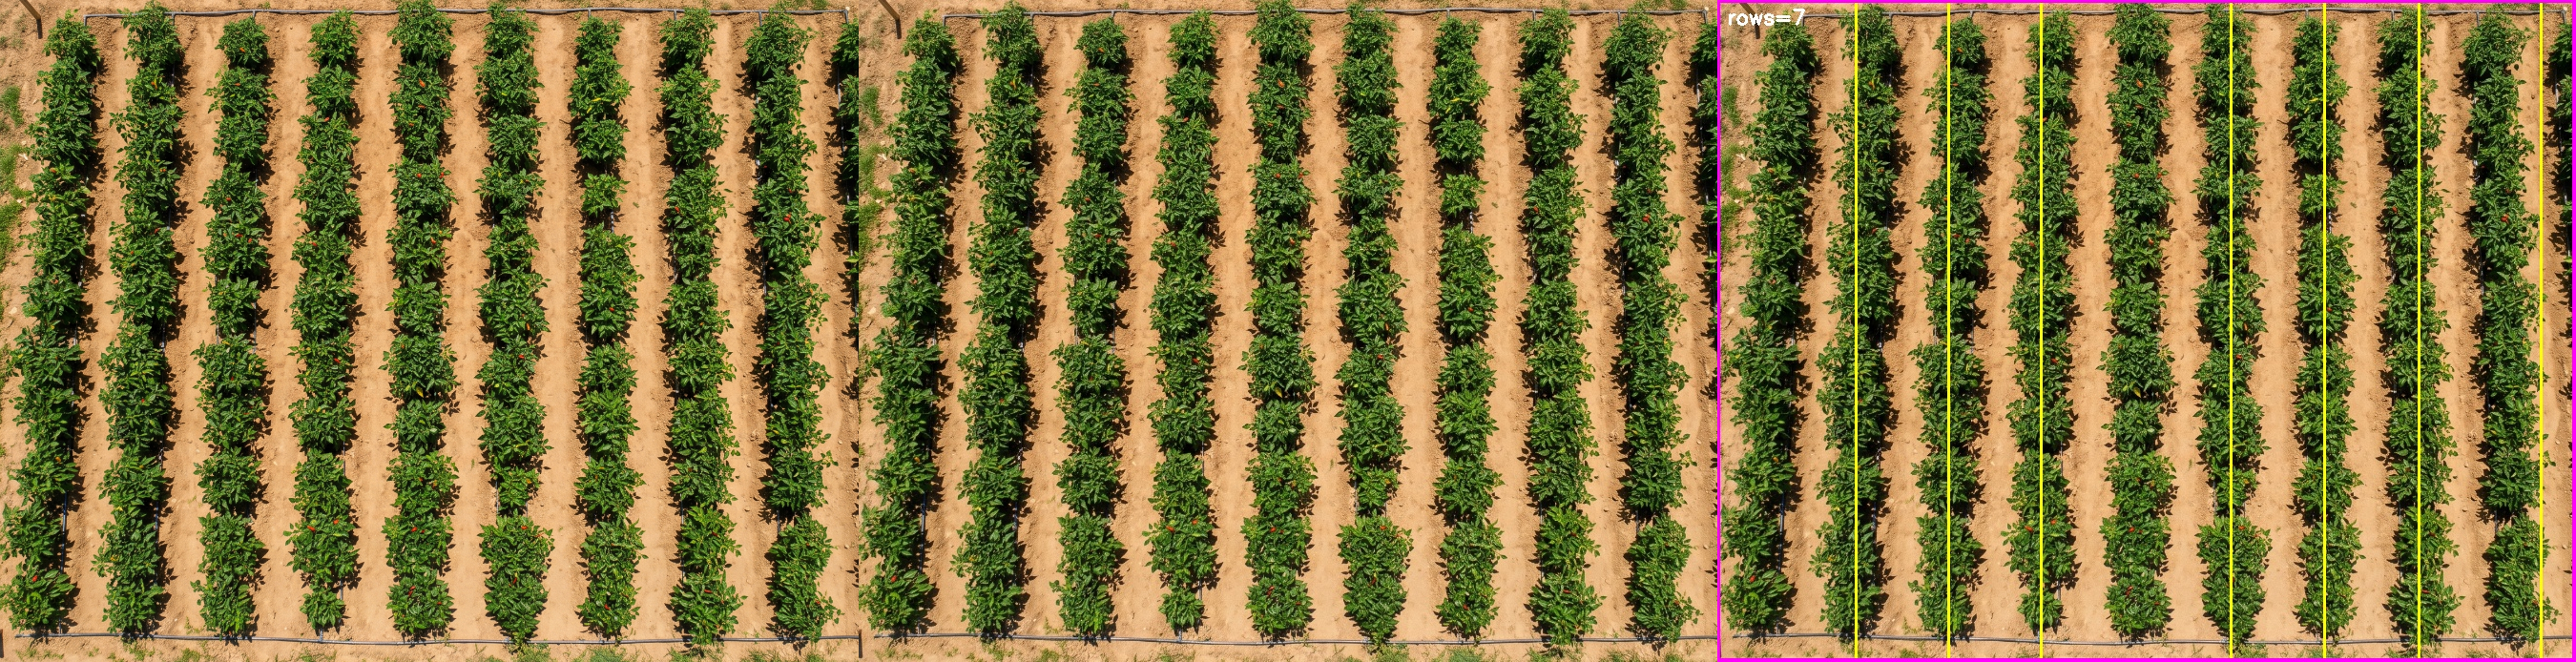
\includegraphics[width=\linewidth]{real_field_triptych.png}
\caption{Real-field pipeline demonstration: (a) smartphone photo of a
seedling block, (b) metric BEV after corner warp, (c) detected rows overlaid
(yellow). 7/7 rows on the tapped block; 19.5\,ms end-to-end.}
\label{fig:realfield}
\end{figure}

Fig.~\ref{fig:example} shows the synthetic-field equivalent at an extreme
$60^\circ$ camera tilt with 0.6\,m row pitch: the raw merged row list
dissolves lost rows that the regularizer recovers.

\begin{figure}[t]
\centering
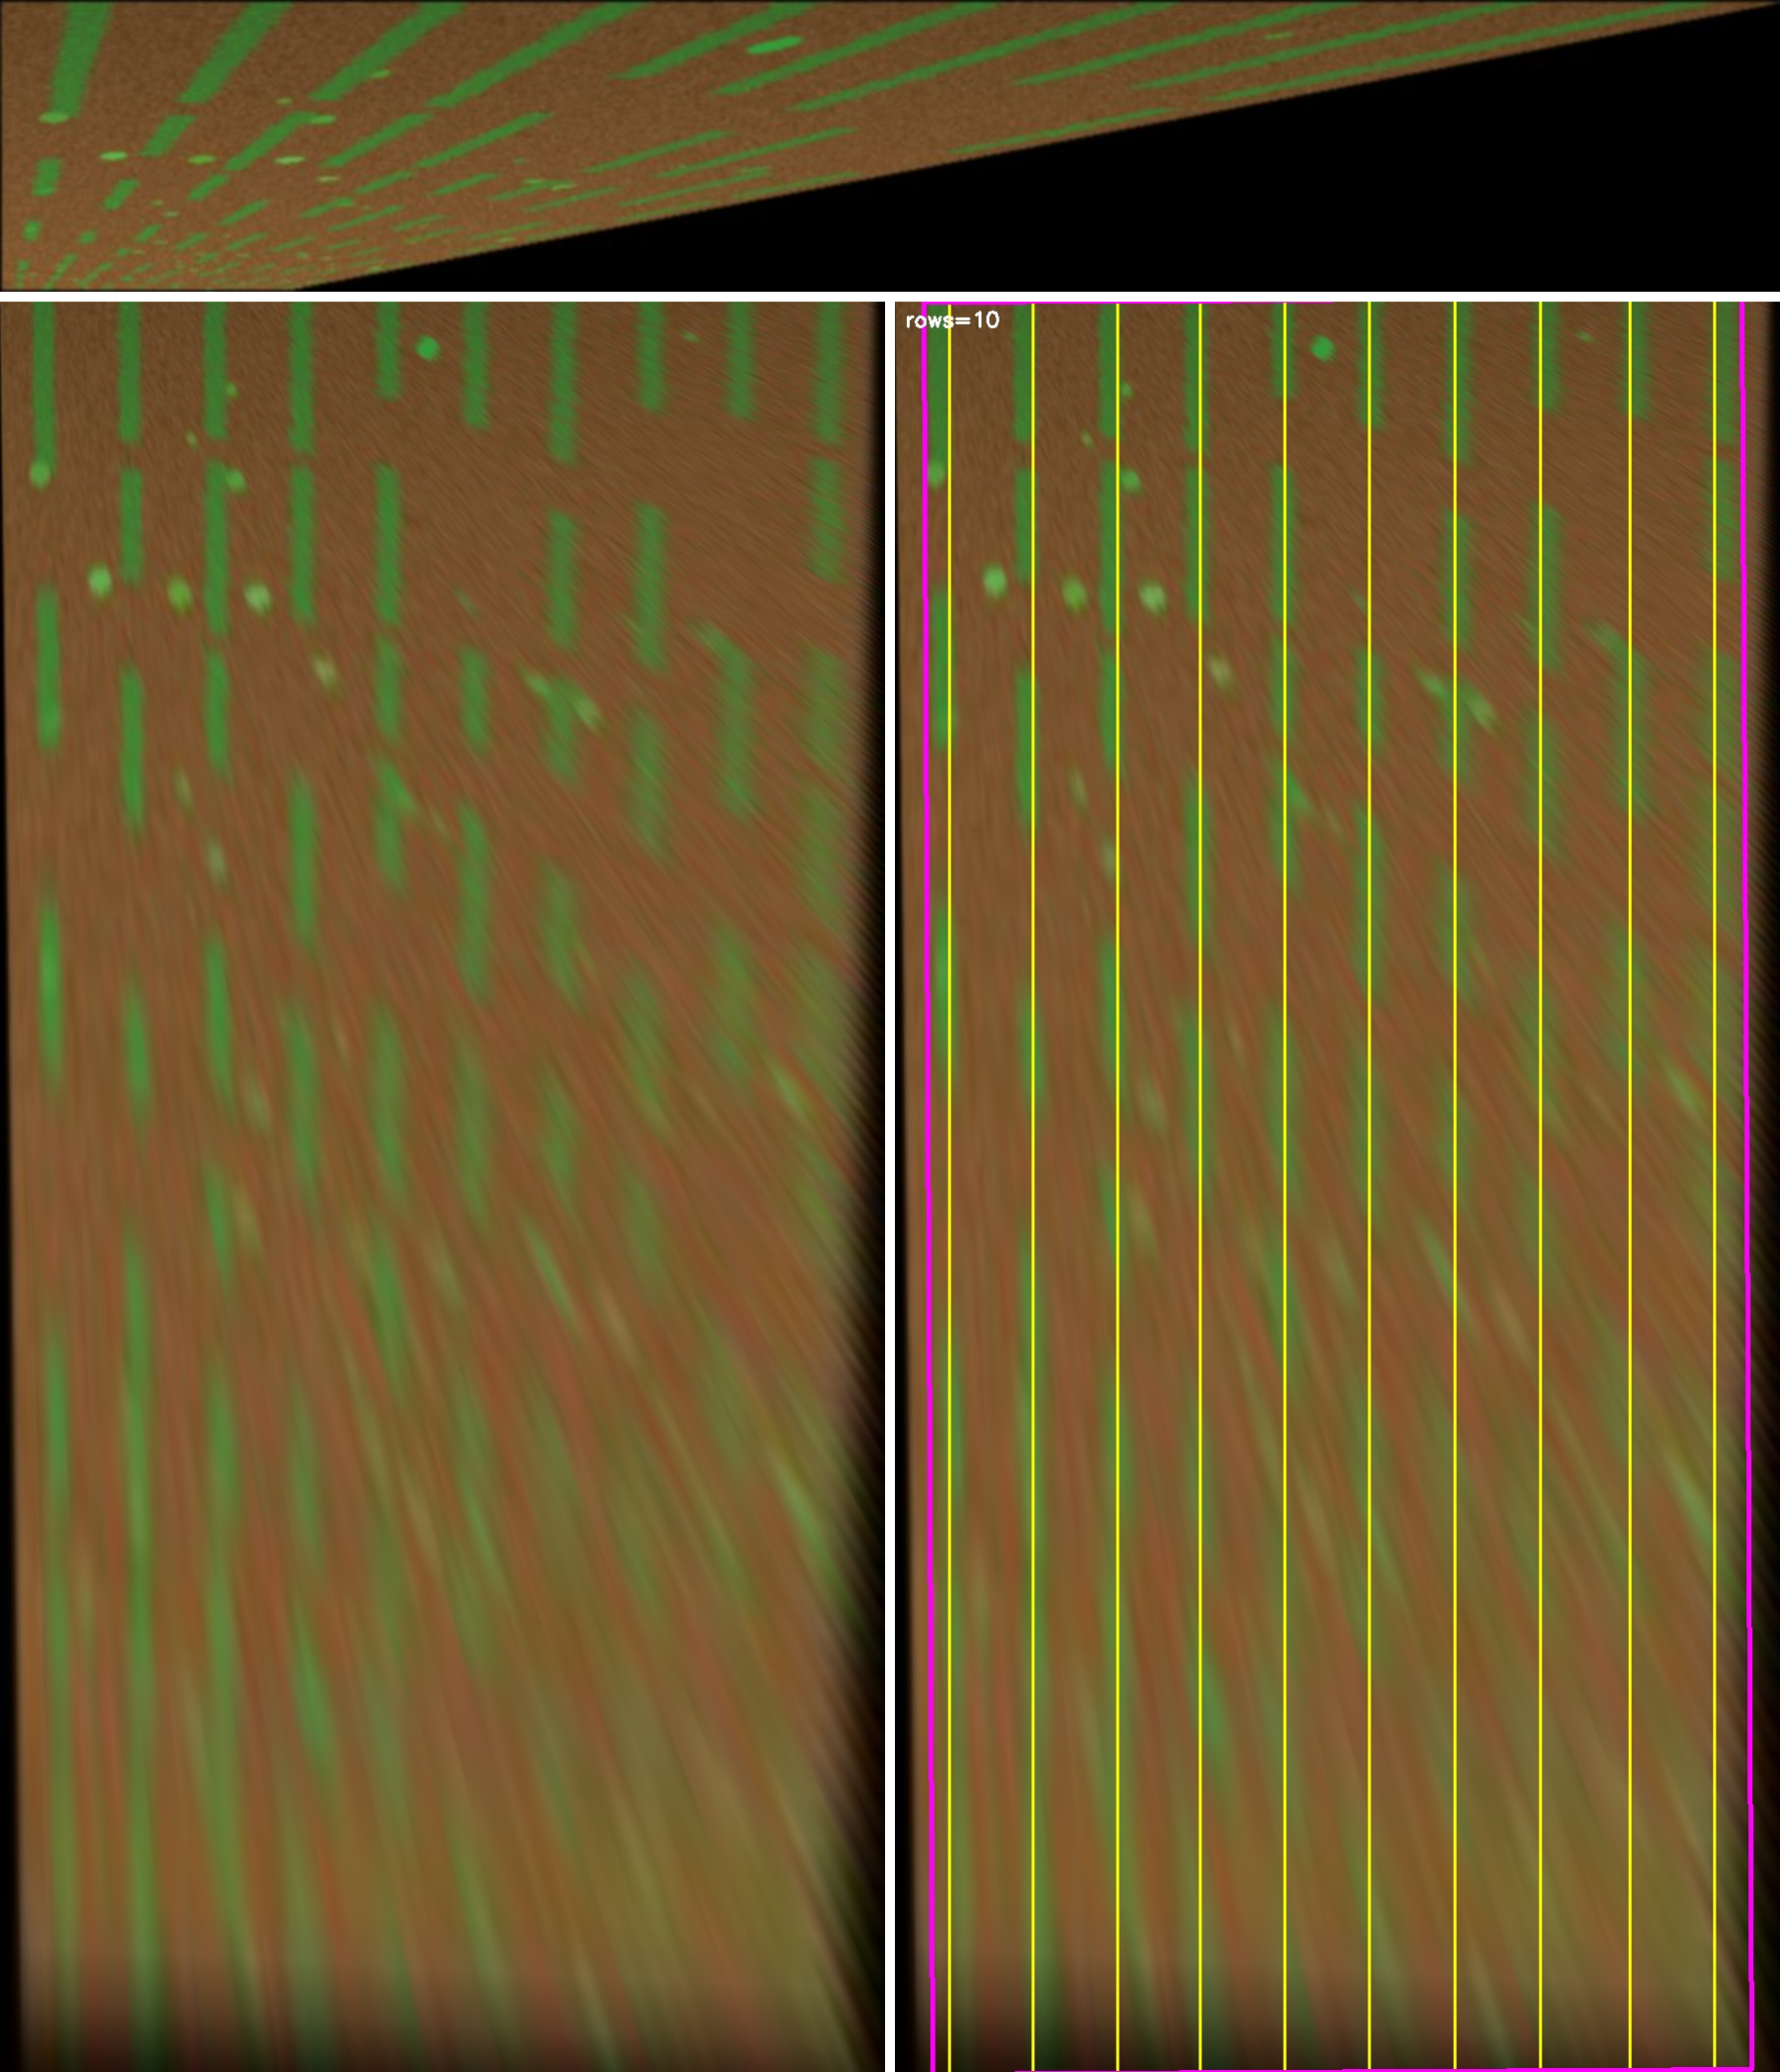
\includegraphics[width=\linewidth]{fig_example.png}
\caption{Synthetic benchmark example at $60^\circ$ tilt, 0.6\,m pitch:
(a) rendered tilted photo, (b) metric BEV, (c) final overlay. Row gaps and
weed clutter make raw projection fragile; regularization restores the
operator-declared row layout.}
\label{fig:example}
\end{figure}

\section{Mission Planning and Execution}\label{sec:mission}

\subsection{Boustrophedon Planning}
Row centers and the field metric dimensions yield a lane-following mission:
each row lane is traversed end-to-end with alternating directions, inset by a
0.2\,m headland margin at both ends (one waypoint per lane end, so a
$k$-row block produces $2k$ waypoints), emitted as plain JSON. Keeping the
mission language JSON and shallow means the same artifact drives the 3-D
twin simulation, the phone app's preview, and the on-board executor without
translation. Fig.~\ref{fig:plan} shows an authentic mission-server output for
a real user upload: nine lane rows and the boustrophedon traversal bounds
computed from the tapped corners.

\begin{figure}[t]
\centering
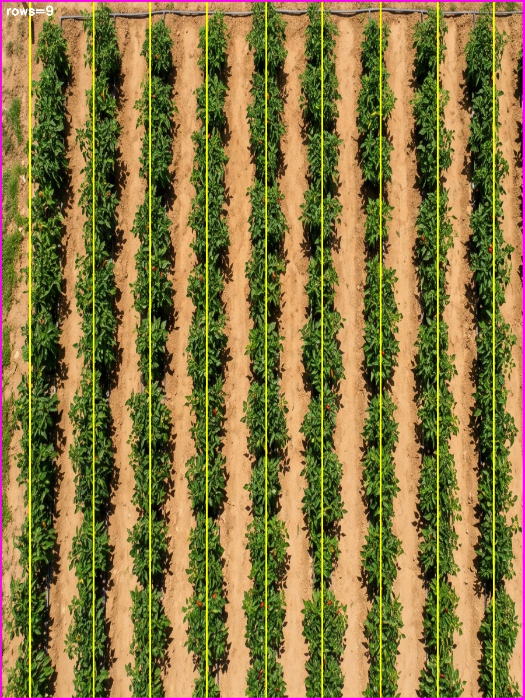
\includegraphics[width=0.85\linewidth]{mission_plan.png}
\caption{Authentic mission-server output for a real field upload: detected
lane rows (yellow) and the traversal bounds (magenta) computed from one
tapped-corner photo upload.}
\label{fig:plan}
\end{figure}

\subsection{Following, Aiming, Zapping}
At run time the executor interleaves lane travel and a head-turn-zap pattern:
the rover drives to waypoints with a differential-wheel controller routed
through the ESP32 (which averages odometry and watches the ultrasonic
stop-sensor), suspends lane travel at each pointing station, aims the arm
using the lane-relative weed coordinates computed from the row map, gates
zap duration to weed width, and remounts. A finite-state machine arbitrates
modes so that perception, navigation, and laser safety never co-drive the
same actuator.

\subsection{3-D Simulation Validation}
Before the hardware ever reached the field, complete missions were replayed
in a Blender-rendered 3-D twin of the rover in which the same mission JSON
drives the same state machine interfacing to a simulated chassis/arm/laser.
Fig.~\ref{fig:sim} shows four frames of a mission replay spanning the
entrance, mid-lane travel, a zap event, and a row-end turn. Because the
simulation consumes the production mission artifact and state machine, it
validates the whole chain from map JSON onward.

\begin{figure}[t]
\centering
\begin{minipage}{0.495\linewidth}
  \centering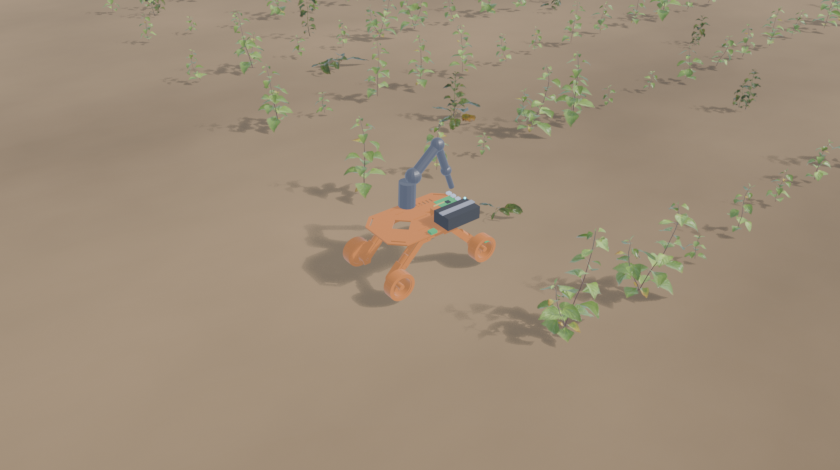
\includegraphics[width=\linewidth]{blender_twin_start.png}
\end{minipage}\hfill
\begin{minipage}{0.495\linewidth}
  \centering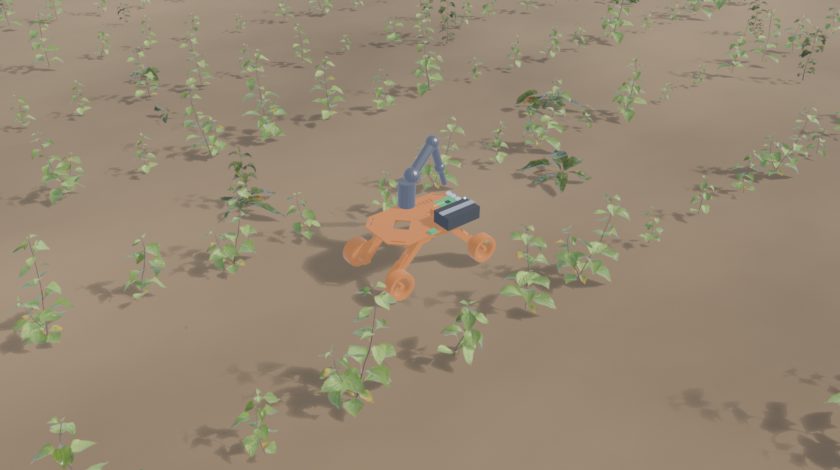
\includegraphics[width=\linewidth]{blender_twin_mid.png}
\end{minipage}\\[1mm]
\begin{minipage}{0.495\linewidth}
  \centering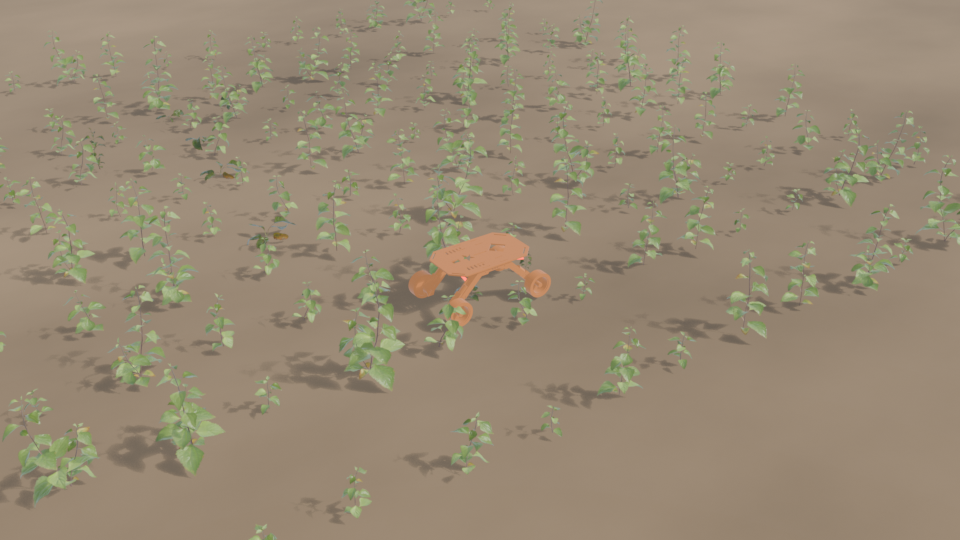
\includegraphics[width=\linewidth]{blender_twin_zap.png}
\end{minipage}\hfill
\begin{minipage}{0.495\linewidth}
  \centering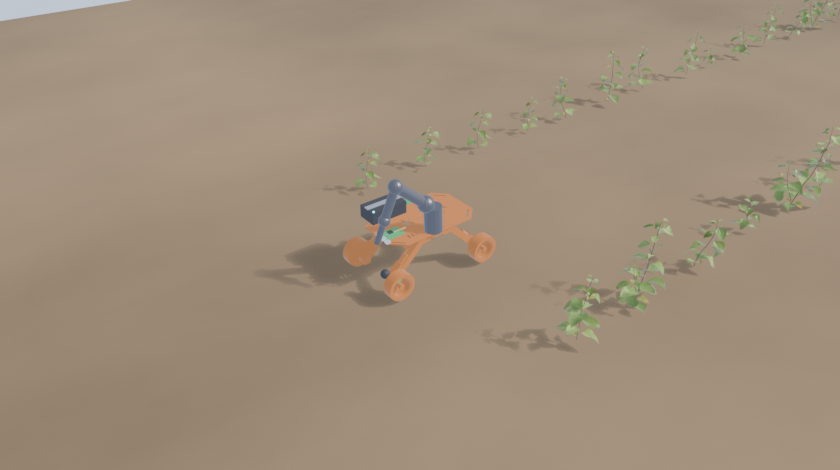
\includegraphics[width=\linewidth]{blender_twin_end.png}
\end{minipage}
\caption{3-D tandem simulation of the physical mission replay: field
entrance (top left), mid-lane travel (top right), laser zap engagement
(bottom left), and end-of-mission (bottom right).}
\label{fig:sim}
\end{figure}

\section{Evaluation}\label{sec:eval}

\subsection{Benchmark Design}
Because no instrumented field trials exist yet, perception robustness is
quantified on a released synthetic benchmark with ground truth
(\texttt{Navigation/benchmarks/}). Fields are generated at
$6\,\mathrm{m}\times12\,\mathrm{m}$ with 100\,px\,m$^{-1}$, containing thin
(0.15\,m) crop bands broken into plant-run segments with realistic gaps, 90
scattered weed blobs, pixel grain, low-frequency soil mottling, and per-trial
random seeding. A pinhole camera model renders each field as if photographed
by a tilted phone: the plane is rotated about the horizontal axis by angle
$\theta$, projected from 2\,m above the near edge, then given a lighting
gradient, mild Gaussian blur, JPEG compression (quality 85), and Gaussian
corner-tap error ($\sigma=3$\,px) added to the four projected corners, which
are passed to the production pipeline as the operator's taps. Each
configuration is run over 8 random seeds.

Two sets are reported: a \emph{tilt sweep} ($\theta \in
[0^\circ..60^\circ]$ step $10^\circ$, both 1.2\,m and 0.6\,m row pitches,
i.e.\ 2 arms $\times14$ settings) and a \emph{tap sweep} ($\sigma \in
[0,2,4,8,16]$\,px at $30^\circ$). An ablation arm disables only the
regularizer, keeping merge and thresholds identical. The complete sweep
comprises 192 pipeline runs. Additional realism stressors are deliberately
modest; no claim is made that synthetic trials substitute for field
validation.

Metrics: row-count error (detected minus expected), exact-count rate, mean
row position error when the count is exact, and mission waypoint-count error.
All timing is measured on an x86-64 laptop (Intel i3-1215U), reported as a
platform-relative reference---the production host is the rover's
single-board computer.

\begin{table}[t]
\caption{Tilt-sweep exact row-count rate (\%) over 8 seeds per cell.}
\label{tab:tilt}
\centering
\begin{tabular}{@{}cc|cc|cc@{}}
\hline
 & & \multicolumn{2}{c|}{1.2\,m pitch} &
   \multicolumn{2}{c}{0.6\,m pitch}\\
Arm & $\theta$ & rate & $|\Delta x|$\,cm & rate & $|\Delta x|$\,cm\\
\hline
raw & $0^\circ$ & 100 & 2.1 & 100 & 1.8\\
raw & $30^\circ$ & 100 & 5.4 & 100 & 4.7\\
raw & $50^\circ$ & 100 & 6.1 & \textbf{75} & 6.9\\
raw & $60^\circ$ & 100 & 7.5 & \textbf{75} & 6.8\\
reg & $0^\circ$ & 100 & 2.1 & 100 & 1.8\\
reg & $30^\circ$ & 100 & 5.4 & 100 & 4.7\\
reg & $50^\circ$ & 100 & 6.1 & 100 & 6.9\\
reg & $60^\circ$ & 100 & 7.5 & 100 & 6.9\\
\hline
\end{tabular}
\end{table}

\subsection{Tilt Robustness}
Table~\ref{tab:tilt} and Fig.~\ref{fig:tilt} show the central result. At
1.2\,m pitch, both arms stay at 100\,\% exact counts at every tilt; the wide
pitch leaves so much projection headroom that even $60^\circ$ cannot collapse
neighboring peaks. At 0.6\,m pitch, the unregularized pipeline merged or lost
rows in 2 of 8 seeds at both $50^\circ$ and $60^\circ$ (mean count error
$-0.25$ and $-0.375$), while the regularized pipeline detected the exact
count in every trial. Two camera-physical mechanisms explain the raw curve's
shape: far-edge ground-sampling-distance inflation (the ratio of near-edge to
far-edge ground resolution reaches $\approx6\times$ at $60^\circ$ for a
12\,m field from 2\,m above the near edge), so blur smears adjacent band
projections together, and gap-driven band thinning, which drops whole rows
below the segment threshold. Regularization repairs both failure modes because
a lost/merged row leaves a predictable hole in a near-uniform grid.

Row position error grows monotonically with tilt in both arms (from
$\approx2$\,cm level at $0^\circ$ to 7.5\,cm at $60^\circ$) because the same
GSD inflation perturbs the mode-center estimate of the far rows; it never
threatens mission validity (bold in Table~\ref{tab:tilt}), and waypoint-count
errors were zero in all trials where the count was exact, and exactly
$\pm$1 lane end per lost row in the raw arm's failed cells.

\begin{figure}[t]
\centering
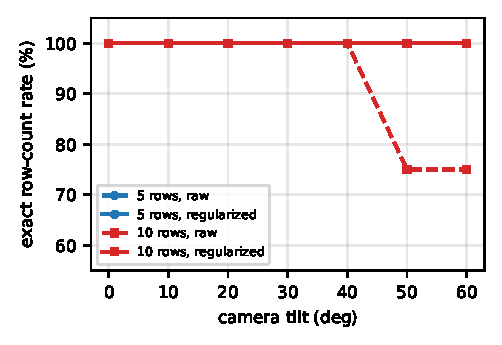
\includegraphics[width=\linewidth]{fig_tilt.pdf}
\caption{Exact row-count rate versus camera tilt for both row pitches and
pipeline variants. The unregularized pipeline (dashed) collapses at
$50$--$60^\circ$ on the 0.6\,m pitch; regularization (solid) stays at
100\,\% throughout.}
\label{fig:tilt}
\end{figure}

\begin{figure}[t]
\centering
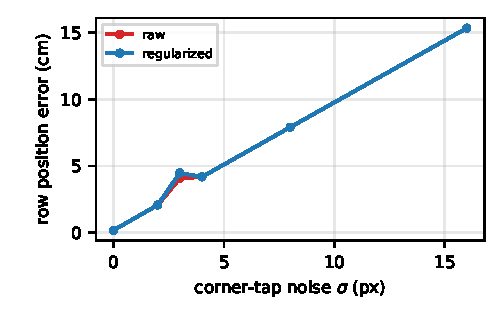
\includegraphics[width=\linewidth]{fig_tap.pdf}
\caption{Row position error versus corner-tap noise at $30^\circ$ tilt
(1.2\,m pitch). Both arms linearly track tap error; the arms coincide
because tap noise perturbs position, not count, on this pitch.}
\label{fig:tap}
\end{figure}

\subsection{Corner-Tap Robustness}
Fig.~\ref{fig:tap} varies the Gaussian corner-tap error at fixed $30^\circ$
tilt. Row position error grows essentially linearly with tap error---from
0.2\,cm at $\sigma=0$ to 15.3\,cm at $\sigma=16$\,px---while row counts and
mission validity remain perfect at both 1.2\,m and 0.6\,m pitch. The
practical reading: casual tapping (a few pixels) costs a few centimeters of
lane alignment, which is far below the row-following tolerance of a
laser pointer of beam width at arm reach.

\subsection{Timing on a Real Photograph}
Table~\ref{tab:timing} reports end-to-end cost on the real photograph of
Fig.~\ref{fig:realfield} (tapped block: 1580$\times$1229\,px $\to$ BEV
$900\times694$\,px; minimum of 7 repeats). Segmentation dominates once
again because it is the only stage processing full color at full
resolution; the projection/regularization chain is negligible
($<2$\,ms). The full-frame photo (both blocks plus surroundings,
2816$\times$1536\,px) processed at 88\,ms end-to-end, confirming that
the sensible strategy of tapping the field block rather than the whole
frame keeps the pipeline well under real-time on the same class of CPU.

\begin{table}[t]
\caption{Real-photo pipeline timing (minimum of 7 repeats, i3-1215U).}
\label{tab:timing}
\centering
\begin{tabular}{@{}lc@{}}
\hline
Stage & Time (ms)\\
\hline
BEV warp & 1.2\\
vegetation segmentation & 7.1\\
projection / merge / regularize & 0.3\\
end-to-end (incl.\ image I/O) & 19.5\\
\hline
\end{tabular}
\end{table}

\section{Limitations}
Three limitations bound the current claims honestly. First, robustness
numbers come from a synthetic benchmark with deliberately modest realism
stressors, not from field trials; the synthetic generator and seeds are
released precisely so that future in-field measurements can be compared
like-for-like. Second, the regularizer trusts the operator's expected row
count; a mis-typed count would snap rows into a wrong (but self-consistent)
grid, which is why the interface polls it explicitly rather than inferring
it. Third, the arm's aiming loop uses the pre-mission row map rather than
per-frame closed-loop vision, so lane-keeping errors during travel add
directly to aim error at resumption; a wrist camera would remove that
coupling.

\section{Conclusion}\label{sec:conclusion}
A complete laser-weeding rover was presented whose entire mission-autonomy
input is one smartphone photograph and four corner taps, processed entirely
on a single-board computer in milliseconds. The central perception
extension---an expected-count row regularizer against a corner-driven BEV
warp---was shown to restore 100\,\% exact row detection where the raw
pipeline falls to 75\,\% under $50$--$60^\circ$ tilt at a realistic 0.6\,m
row pitch, and the system was validated end-to-end in a 3-D tandem
simulation using the same production mission artifacts and state machine as
the hardware, plus a working chassis prototype and a connectivity-clean
KiCad electrical design. The natural next steps are instrumented field
trials on the synthetic benchmark's conditions, weed-level (not row-level)
targeting with per-stem aim, and an on-board wrist camera for closed-loop
aiming between lane stations.

\section*{Acknowledgment}
The author thanks the open-source community behind OpenCV, NumPy, KiCad,
and Blender. An AI coding assistant was used during development for
code drafting and review, benchmark tooling, documentation, and manuscript
preparation; the author personally directed the engineering work, verified
all reported results independently, and takes full responsibility for the
content of this paper.

\bibliographystyle{IEEEtran}
\begin{thebibliography}{9}

\bibitem{oerke2006} E.-C. Oerke, ``Crop losses to pests,'' \emph{J. Agric.
Sci.}, vol. 144, no. 1, pp. 31--43, 2006.

\bibitem{astrand2002} B. \AA strand and A.-J. Baerveldt, ``An agricultural
mobile robot with vision-based perception for mechanical weed control,''
\emph{Auton. Robots}, vol. 13, no. 1, pp. 21--35, 2002.

\bibitem{ruckelshausen2009} A. Ruckelshausen \emph{et~al.}, ``BoniRob---an
autonomous field robot platform for individual plant phenotyping,''
in \emph{Precision Agriculture '09}. Wageningen, The Netherlands, 2009.

\bibitem{wu2020} X. Wu, S. Aravecchia, P. Lottes, C. Stachniss, and
C. Pradalier, ``Robotic weed control using automated weed and crop
classification,'' \emph{J. Field Robot.}, vol. 37, no. 2, pp. 322--340,
2020.

\bibitem{gao2026} F. Gao \emph{et~al.}, ``A review of robotic weeding
modalities for site-specific weed management,'' \emph{Sensors},
vol. 26, no. 10, 2925, 2026.

\bibitem{woebbecke1995} D. M. Woebbecke, G. E. Meyer, K. von Bargen, and
D. A. Mortensen, ``Color indices for weed identification under various soil,
residue and lighting conditions,'' \emph{Trans. ASAE}, vol. 38, no. 1,
pp. 259--267, 1995.

\bibitem{otsu1979} N. Otsu, ``A threshold selection method from gray-level
histograms,'' \emph{IEEE Trans. Syst., Man, Cybern.}, vol. SMC-9, no. 1,
pp. 62--66, 1979.

\bibitem{carbonrobotics} Carbon Robotics, ``LaserWeeder'' [Online].
Available: \url{https://www.carbonrobotics.com}

\end{thebibliography}

\end{document}
